\documentclass[UTF8]{beamer} 
\usepackage{ctex}
\usepackage{Sweave}
\usetheme{Boadilla} 
\usepackage{color} 
\usepackage{graphicx} 

\begin{document}

\title{R编程与进化分析} 
\subtitle{第一部分 R编程}
\author{张金龙} 
\institute{jinlongzhang01@gmail.com}
\date{2016年5月9日 北京} 

\frame{\titlepage} 
\section{R开发平台}

\begin{frame}
\frametitle{目录}
\tableofcontents
\end{frame}

\begin{frame}
\frametitle{目录}
\tableofcontents[currentsection] 
\end{frame}

\frame{
    \frametitle{善其事, 利其器}
        \begin{itemize}
    \item R
    \item Rtools
    \item MikTeX/TexLive
    \item Editors(Notepad++, Geany)
    \item Rstutio
    \item Console/Terminal/Rcmd/Rscript
        \end{itemize}
}

\frame{
    \frametitle{R in Console/Terminal}
    \begin{center}
    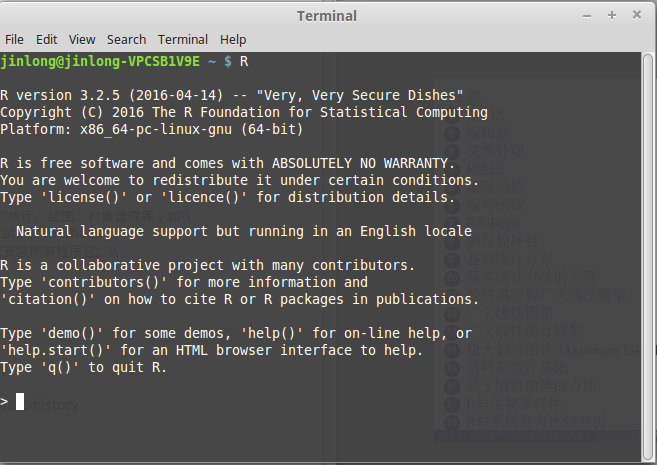
\includegraphics[height=2.5in]{Selection_053.png}\\
    \medskip
    
    \end{center}
}

\frame{
    \frametitle{R代码编辑器的基本要求}
作为一个好的脚本编辑器, 需要满足以下要求:\\
1. 代码的高亮显示\\
2. 括号匹配\\
3. 不能随便更改大小写\\
4. 方便查找和替换\\
5. 以列的方式批量进行输入, 特别是列\\
6. 等宽字体,便于对函数结构进行缩进, 如Courier New, Consolas\\

}

\frame{
    \frametitle{Notepad ++ 对R代码的高亮显示}
    \begin{center}
    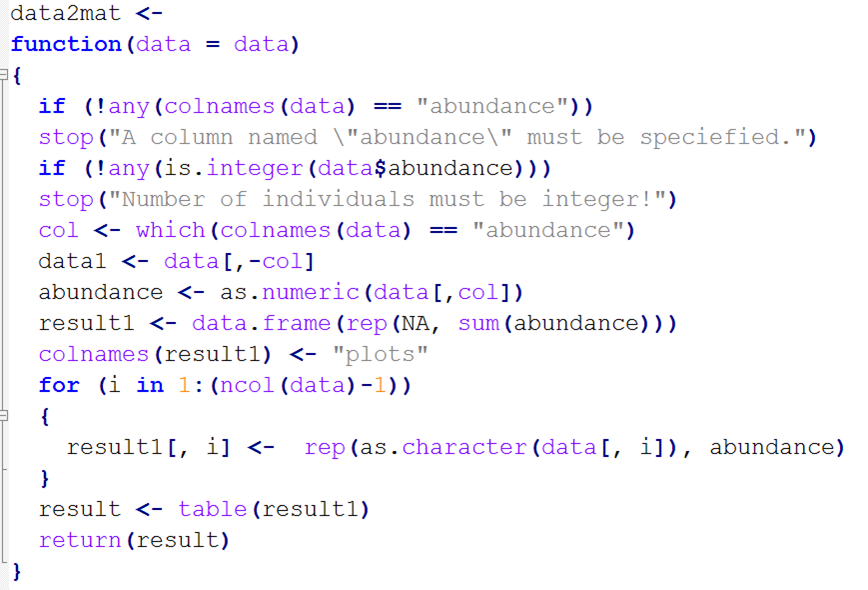
\includegraphics[height=2.5in]{highlight.png}\\
    \medskip
   关键词显示为不同颜色, 可以找到匹配的括号。 
    \end{center}
}

\frame{
    \frametitle{推荐的开发环境 \\
   1.  Rstudio Integrated Development Environment (IDE)}
    \begin{center}
    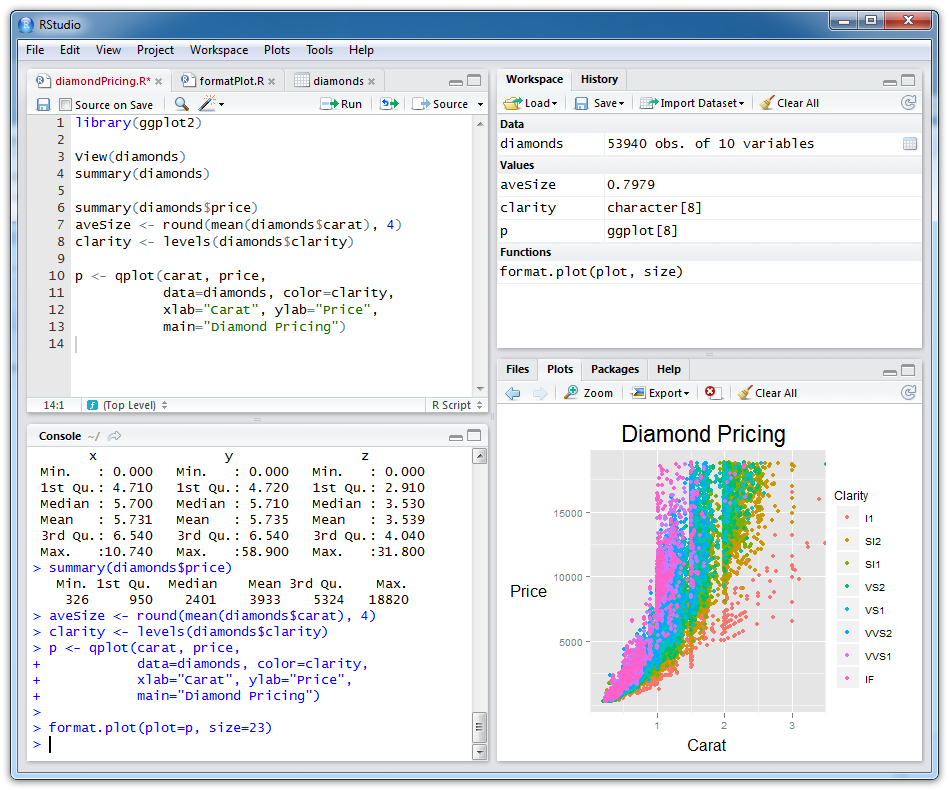
\includegraphics[height=2.5in]{rstudio.png}\\
    \medskip
    Rstudio, available on Linux, Windows, MacOS\\
    \end{center}
}

\frame{
    \frametitle{2. Notepad++ 或 geany }
    \begin{center}
    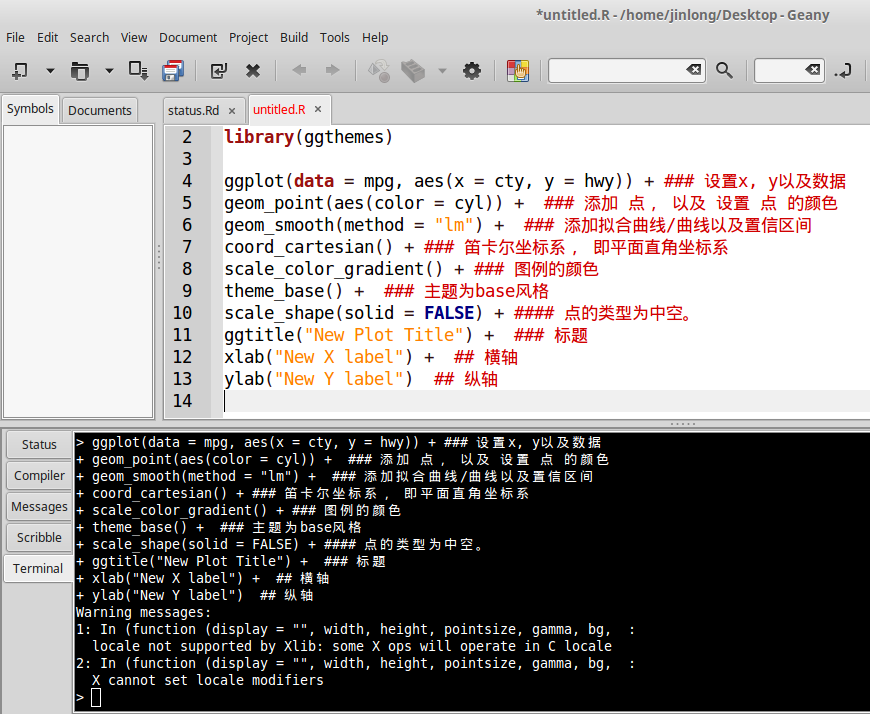
\includegraphics[height=2.5in]{Selection_054.png}\\
    \medskip
    编辑代码十分灵活, 批量运行代码
    \end{center}
}

\frame{
    \frametitle{R脚本的主要内容}
    \begin{itemize}
\item 1. 设定工作路径\\
\item 2. 导入所需要的程序包\\
\item 3. 定义所需要的部分函数\\
\item 4. 数据的读取\\
\item 5. 数据的操作和绘图等\\
一般在最开始时, 还需要加上标题, 日期, 作者等。 便于查阅\\
    \end{itemize}
}


\frame{
    \frametitle{编写R脚本的注意事项}
    \begin{itemize}
\item 1. 打开高亮显示, 括号配对\\
\item 2. 缩进,因此一定要用等宽字体(如Consolas
Courier New等), 并且用空格缩进, 少用tab缩进\\
\item 3. 变量名要长,意义要清晰, 最好看到变量名, 就知道该变量的意义\\
\item 4. 少用., 多用\_\\
\item 5. 括号成对书写\\
\item 6. 有详细的注释\#
    \end{itemize}
}

\frame{
    \frametitle{编程习惯:编写好的R脚本I}

好的R脚本: 目标明确, 结构清晰, 容易阅读, 容易理解, 容易维护。

理想情况是, 不看注释, 只看变量名, 也能读懂代码的结构和含义。

 \begin{itemize}
    
\item 所有的R脚本, 以应R作为扩展名,以便打开后默认为R的高亮显示. 
\item R脚本建议开头写标题, 作者, 日期, 联系方式. 
\item 按照顺序安排 (1)setwd(), 指定工作目录,工作目录最好不要有中文, (2)加载程序包, (3)定义新的函数
\item 变量的名称要具体,并且只用英文字母以及数字编写, 不能用中文。
\item 不用Tab,只用英文空格。在 赋值符号前后 <- 都要增加一个空格。

\end{itemize}
}


\frame{
    \frametitle{编程习惯:编写好的R脚本II}

 \begin{itemize}
\item 变量名要有具体的意义, 最好用英文,除了循环变量 i, j, n, k, 必须避免A,X等单个字母的变量名。 尽量不要大小写混搭, 不同部分用下划线分隔。 
\item 算法的关键部分, 要注释, 特别容易出错的地方也要注释。
\item 缩写的函数要简单明确, 以方便维护. 
\item 脚本可以从开始直接运行到结束, 而无需手动输入数值,或者手动保存文件
\end{itemize}
更多请参考 Google R编程指南
}

\frame{
    \frametitle{演示以及问题: 编程习惯}
    你在编写R脚本时有什么好的或者坏的习惯?
 }

%#############################################################
\section{编写函数}
\begin{frame}
\frametitle{目录}
\tableofcontents[currentsection] 
\end{frame}


\frame{
    \frametitle{代码的重用:为什么要编写函数}
mat是输入的群落数据矩阵\\
\begin{block}{计算shanon生态位宽度的R代码}
{\tt
Bi $<-$ c()\\
for (i in 1:ncol(mat)) \{\\
nij $<-$ mat{[, i]}\\
nij $<-$ nij{[nij $>$ 0]}\\
pij $<-$ nij/sum(nij)\\
Bi{[i]} $<-$ -sum(pij $\star$ log(pij))\\
\}
Bi $<-$ as.data.frame(t(Bi))\\
colnames(Bi) $<-$ colnames(mat)} \\
\end{block}
Bi是计算结果。 \\
问题: 每次计算shannon生态位宽度, 都要拷贝这段代码?\\

代码的重复拷贝, 不但浪费了大量的时间和精力, 而且非常容易产生错误, 并且难以纠正。 \\
}


\frame{
    \frametitle{编写R函数}
   \begin{itemize}  
\item 1. 函数名称,即要编写的函数名称,这一名称就作为将来调用R函数的依据。
\item 2. 函数声明,包括  <- function, 即声明该对象的类型为函数。
\item 3. 函数参数,定义函数时输入的数据,只是一种形式, 定义函数时并不运行函数本身,所有参数只是形式上存在, 即形式参数,简称形参。 函数体内部的语句进行数据处理,就是对参数的值进行处理 ,这种处理只在调用函数的时候才会发生。所以, 实际输入的参数, 称为实际参数, 简称实参。 R帮助文件对每个R函数的参数都进行了说明。 
\item 4. 函数体: 进行参数检查, 数据处理, 以及定义返回值。 
\end{itemize}
}

\frame{
    \frametitle{编写R函数:函数体}
       \begin{itemize} 
       \item (1). 异常处理: 对输入的参数进行检查, 包括类型, 值域
       \item (2). 算法: R是向量语言, 应该尽量减少用for循环
       \item (3). 返回值, 只允许有一个返回值
       \end{itemize}
}

\frame{
    \frametitle{R函数}
编写R函数是减少代码重复拷贝,提高程序效率的重要手段。\\
R可以方便地编写函数,用户编写的函数可以直接调用。\\
R编写函数时, 无需声明变量的类型,这与C,C++等语言不同。\\
\medskip
\begin{block}{R函数基本结构}
   函数名 $<-$ function(数据,参数1= 默认值,参数2= 默认值,…)\{ \\
          异常处理;\\
          表达式(循环/判别);\\
          return(返回值);\\
       \}
\end{block}
}

\frame{
    \frametitle{R函数:时分秒转换成十进制}
\begin{block}{函数举例}
{\tt
deg2dec $<-$ function (h, m, s) \{\\
    if(any(!is.numeric(c(h,m,s))))\{\\
        stop("None numeric value find, can not calculate")\\
    \}\\
    if (h < 0) \{\\
        m = -m\\
        s = -s\\
    \}\\
    res = h + m/60 + s/3600\\
    return(res)\\
\}}\\
\end{block}
deg2dec(23,56,04)\\
deg2dec(23,56,"Test")\\
}

\frame{
    \frametitle{for循环和while循环}
    for是循环中最重要的函数之一, 在for循环下, 只要条件满足, 即执行后面花括号\{\}内的语句,如果是只有一行语句, 则花括号可以省略。 \\
for(变量 in 向量) 表达式\\

\begin{block}{for的用法}
dat $<-$ rpois(20,19)\\
for(i in 1:20) \{\\
print(dat[i])\\
\}\\
\end{block}
while循环是满足条件下,执行某些语句的控制函数。
\begin{block}{while的用法}
i $<-$ 1\\
while(i$<$10)\{ \\
print(i);  \\
i $<-$ i + 1\\
\}
\end{block}

}

\frame{
\frametitle{流程控制if}
if是在条件为真的情况下, 执行后面程序的条件控制语句。决定程序的分支和走向\\
\begin{block}{if的用法}
if(条件) \{表达式\} \\
if(条件) \{表达式1\} else \{表达式2\} \\
\end{block}
\begin{block}{if举例}
p $<-$ 0.03 \{\\
if(p $<=$ 0.05) \{ \\
   print("p $<=$ 0.05\!")\\
\} else  \{\\
   print("p $>$ 0.05\!")\\
\}\\
\}
\end{block}
}


\frame{
    \frametitle{用warning和stop处理异常}
若数据格式等不能满足要求,或者参数设定错误,函数处理往往会给出错误的结果,此时,必须发出警告或及时终止程序,以提高程序的稳健性。\\
\begin{block}{警告的写法}
{\tt if(any(is.na(inputdata)))\\
inputdata $<-$ na.omit(inputdata)\\
cat($''$NAs found in the input data, and have been removed.$''$)}\\
\end{block}
\begin{block}{终止的写法}
 {\tt if(any(is.na(xx))) stop($''$NAs are not allowed!$''$)}\\
\end{block}
\begin{tabular}{ll}
{\color{blue}\textbf{missing()}} &判断某个参数是否缺失, 返回值为TRUE或者FALSE\\
{\color{blue}\textbf{stopifnot()}} &如果不满足某条件, 则中止。\\
\end{tabular}
}


\frame{
    \frametitle{参数的匹配}
\begin{block}{match.arg的使用}

{\tt center $<-$ function(x, type = c("mean", "median", "trimmed")) \\
 \{\\
  type $<-$ match.arg(type)\\
  switch(type,\\
         mean = mean(x),\\
         median = median(x),\\
         trimmed = mean(x, trim = .1))\\
\}
}
\end{block}
type参数在经过match.arg函数处理后,无需输入全称, 即可判断。\\
如果输入的参数和type预设的名称不符, 则触发错误。R给出相应的提示。\\
}


\frame{
    \frametitle{变量的作用域}
输入一个字符串, 如“ABCDE”, 返回“EDCBA”\\

\begin{block}{函数举例}
{\tt 
reverse $<-$ function (x) \\
\{\\
    splitstr $<-$ substring(x, 1:nchar(x), 1:nchar(x))\\
    result $<-$ paste(splitstr{[length(splitstr):1]}, collapse = "")\\
    return(result)\\
\}
}
\end{block}

x为形参,实际参数是输入的结果, 而x的值, 仅在函数的花括号内部生效, 在调用的过程中创建,其他函数不能直接访问x。 随着该函数运行结束, x的值从内存中清除, 这就是x的作用域。\\
}

\frame{
    \frametitle{返回值}
\begin{itemize}
\item 1. 返回值表示函数输出的结果。\\
\item 2. 返回值必须是一个对象。如果函数的结果需要返回多个值,可以创建一个list(),并返回该list。\\
\item 3. R默认将最后一行作为返回值。\\
\item 4. 一个函数内部, 可能出现若干个return()。 如果执行中遇到任意一个return(),函数都将结束, 返回return内部的对象。\\
\end{itemize}
}


\frame{
    \frametitle{Debugging:检查函数的错误}
一般容易出错地方: \\
1. 检查拼写, 括号和运算符等的中英文切换 \\
2. 参数不匹配\\
3. 向量或者矩阵等下标出界\\
4. 逻辑错误(最难发现的错误!)\\
\begin{block}{undebug函数和debug函数}
debug和undebug一定要配合使用。 debug内部放函数名称, 之后再运行该函数时, 函数会一步一步执行, 执行每一步,都需要按回车, 中间过程的变量也都可访问, 因此方便检查错误。 修改完错误后, 一定要用undebug取消debuging.\\
\end{block}
}

\frame{
    \frametitle{Debug和Undebug的用法}
\begin{block}{Debug示例}
{ \tt
print.mat2 $<-$ function(x)\{\\
Ncol $<-$ ncol(x); Nrow $<-$ nrow(x)\\
temp $<-$ c()\\
k = 1\\
for(i in 1:Nrow) \{\\
   for(j in 1:Ncol)\{\\
       temp{[k]} $<-$ x[i,j]\\
       k = k + 1\\
   \}\\
\}\\
return(temp)\\
\}\\
debug(print.mat2)\\
x1 $<-$ matrix(1:20, 4, 5)\\
print.mat2(x1)\\
}
\end{block}
}

\frame{
    \frametitle{演示以及问题: 编写函数进行摄氏度以及华氏度的转换}
	摄氏度到华氏度公式 [°F] = [°C] × 9⁄5 + 32\\
	华氏度到摄氏度公式[°C] = ([°F] − 32) × 5⁄9\\
 }

%%%% ###############################
\section{程序包}
\begin{frame}
\frametitle{目录}
\tableofcontents[currentsection] 
\end{frame}


\frame{
    \frametitle{R 程序包}
    R程序包是一系列R函数的组合,大部分函数都有详细的说明文件。对于R程序包的源代码来说, 要包括以下几个文件 DESCRIPTION和NAMESPACE 两个文本文件,以及如下文件夹:
     \begin{itemize}
     \item R: 用于存放R的函数, 每个函数一个文本文件, 以.R作为扩展名
     \item src:用于存放C, CPP或者FORTRAN等的源代码。
     \item data:扩展名为.rda的二进制文件,常用于函数的Example中。
     \item man: 存放R函数以及数据的说明文件,文件格式为扩展的Latex。 
     \item vignettes, 用来存放Latex编写的程序包说明,还包括用到的图形等。 
    \end{itemize} 
    
   程序包可以放在 CRAN以及R forge, bioconductor 和github上等。
    }

\frame{
    \frametitle{CRAN:The Comprehensive R Archive Network}
CRAN是R的网络镜像网站,类似的 PERL:CPAN;TeX: CTAN;S+: CSAN \\

    \begin{center}
    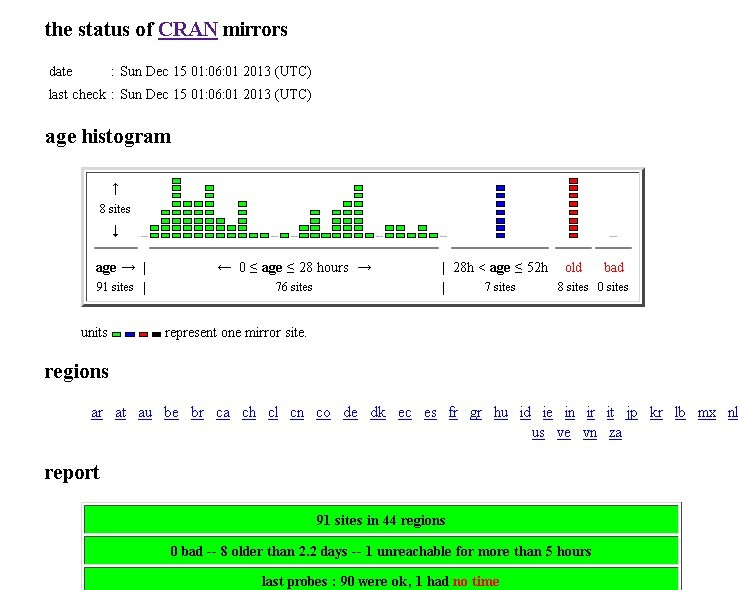
\includegraphics[height=2.0in]{CRAN2.png}\\
    目前有131个镜像网站,分布在44个国家地区(2016-5-1)\\
    每个镜像上, 都可以下载到R的源代码, MacOS, Windows和部分Linux版本的可执行安装文件,以及程序包。\\
    \end{center}
}


\frame{
    \frametitle{CRAN Task Views}
    安装某一类程序包:
    \begin{block}{R code}
    {\tt install.packages("ctv") \#安装ctv程序包\\
    library("ctv")\#导入ctv程序包\\
    install.views("Phylogenetics")\#安装系统发育相关的所有程序包\\
    install.views("Environmetrics")\#安装生态学相关的所有程序包\\
    }
    \end{block}
    \begin{itemize}
    \item Phylogenetics      \\
    \item Multivariate       \\
    \item Bayesian statistics\\
    \end{itemize}
}



\frame{
\frametitle{系统进化常用程序包}
CRAN上, 目前保存了8348个程序包(截至2016年5月1日)\\
按照功能的不同, 在CRAN Task View上, 将程序包的功能按照33个领域分别介绍, 如生态学、空间分析、经济学、社会学、贝叶斯统计、系统发育比较分析等,各领域有专人负责更新。\\
例如系统发育比较分析常用的程序包, 在Phylogenetics这个领域下:\\
    \medskip
    \begin{tabular}{ll}
    
 {\color{blue}\textbf{adephylo}}            &系统发育比较分析 \\
 {\color{blue}\textbf{ape (core)}}          &系统发育与进化分析 \\
 {\color{blue}\textbf{BAMMtools}}         & 贝叶斯方法进行分化速率分析\\
 {\color{blue}\textbf{BioGeoBEARS}}    & 祖先分布区推断\\
 {\color{blue}\textbf{caper}}                 &用R进行系统发育比较分析 \\
 {\color{blue}\textbf{diversitree}}         & 分化速率分析\\
 {\color{blue}\textbf{geiger}}                & 分化速率分析 \\

    \end{tabular}
}

\frame{
\frametitle{系统进化常用程序包II}
    \begin{tabular}{ll}
 {\color{blue}\textbf{ggplot2}}        & 图层化绘图 \\
 {\color{blue}\textbf{ggtree}}          & 图层化绘制进化树\\
 {\color{blue}\textbf{ouch}}             & 性状进化的Ornstein-Ulenbeck模型参数估计\\
 {\color{blue}\textbf{phangorn}}     & 进化树推断等\\
 {\color{blue}\textbf{phyloclim}}     & 气候适应性变化\\
 {\color{blue}\textbf{PHYLOGR}}     &系统发育相关的统计分析 \\
 {\color{blue}\textbf{phytools}}       & 系统发育比较分析程序包\\
 {\color{blue}\textbf{picante}}         & 群落系统发育程序包\\
 {\color{blue}\textbf{Rphylip}}         & Phylip的R界面\\
 {\color{blue}\textbf{taxize}}           & 物种的分类位置查询\\
 {\color{blue}\textbf{TESS}}             & 分化速率推断 \\
 {\color{blue}\textbf{vegan}}           & 群落生态学数据分析\\
    \end{tabular}
}



\frame{
    \frametitle{R forge}
https://r-forge.r-project.org/ \\
部分程序包依靠Rforge保存源代码。\\
R的程序员可以在自己的计算机上开发R程序包, 并且用SVN软件(如Tortoise SVN)同步到Rforge上。 Rforge保存最新版本,以及更改历史, R程序包经检查无误后可以提交到CRAN上。 
}

\frame{
    \frametitle{Github}
https://www.github.com \\
github是发布程序源代码, 以及保存版本历史的网站。github能够与git很好的兼容。 
github上的程序包可以通过devtools程序包安装。 
 \begin{center}
    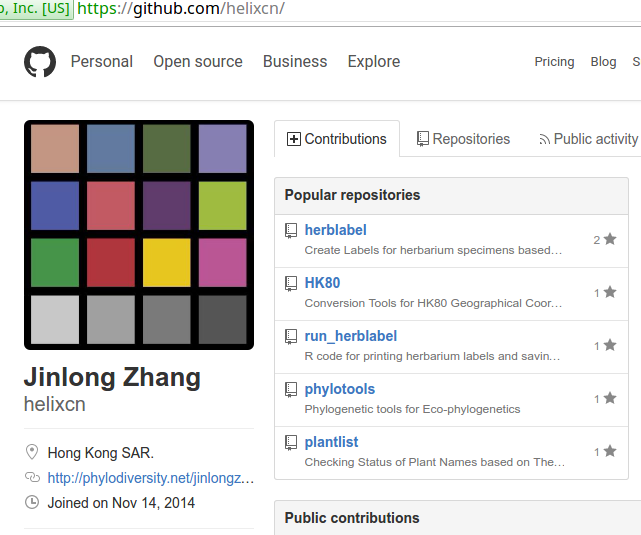
\includegraphics[height=2.5in]{Selection_004.png}\\
    \medskip
    \end{center}

}

\frame{
    \frametitle{版本控制工具Git}
git是版本控制工具, 能够追踪对文件所做的任何修改。\\
因为程序的开发是不断发现错误之后修订错误的过程, 因此版本的控制显得十分重要。 git具有分支开发功能,每个人可以对各自的分支进行修改, 然后合并到master分支上。 \\

 \begin{center}
    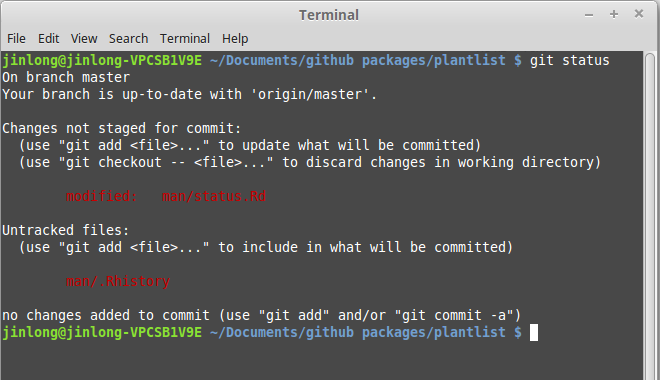
\includegraphics[height=2.in]{Selection_010.png}\\
    \medskip
    \end{center}
}

\frame{
    \frametitle{git:克隆github上的程序包, 并推送更改}
       \begin{itemize}  
\item {\tt git clone https://www.github.com/helixcn/phylotools\\}
\item {\tt git status\\}
\item { Some changes\\}
\item {\tt git status\\}
\item {\tt git commit -m $''$This is an test$''$\\}
\item {\tt git push\\}
\item {\tt git pull\\}
    \end{itemize}  
 }



%%%% #####################################

\section{面向对象编程 S3 和 S4 Methods}

\begin{frame}
\frametitle{目录}
\tableofcontents[currentsection] 
\end{frame}

\frame{
    \frametitle{面向对象编程 Object Oriented Programming    }
什么是面向对象?\\
根据数据的结构不同, 计算机自动选择对应的数据处理方法。对象的属性同时能够传递, 以便更方便得处理, 这种编程思想称为面向对象编程\\
绘图时, 有些数据R会绘制散点图, 有些会绘制boxplot, 有些会绘制成进化树, 就是根据数据的结构不同, 分别用不同的函数处理。 但是在调用的时候,都是用plot函数,这里的plot函数, 称为泛型函数 generic function\\
而真正执行任务的是, 是诸如 \\
{\color{blue}\tt{    plot.default}}\\
{\color{blue}\tt{    plot.density}}\\
{\color{blue}\tt{    plot.lm}}\\
{\color{blue}\tt{    plot.phylo}}\\
等函数。 这些函数称为子函数。这种面向对象的处理方式称为S3 Method。
}

\frame{
    \frametitle{S3 Method  }


\begin{block}{S3类型变量的创建与继承}
x <- 10\\
class(x) \# "numeric"\\
oldClass(x) \# NULL\\
inherits(x, "a") \#FALSE\\
class(x) <- c("a", "b")\\
inherits(x,"a") \#TRUE\\
\end{block}

更多信息请参考 

{\color{blue}\tt{   ?Classes  }}\\
{\color{blue}\tt{   ?Methods }}\\
{\color{blue}\tt{   ?UseMethod}}\\

    S3 Method是一种较为松散自由的面向对象编程, S3的对象中, 对象的类型可以通过class函数随意指定, 这就增加了出错的风险。同时, S3 Method缺少更为稳健和严格的查错机制。为此, Chambers等人研发了更为严格的S4 Method\\
    
}


\frame{
    \frametitle{S4 Method}
    \begin{block}{S4 Method对象的创建以及访问}

    S4 Method 
    
    \#\#\# 创建S4类型的对象, 以及访问内部的数据\\
setClass("Person",slots=list(name="character",age="numeric"))\\
father <- new("Person",name="F",age=44)\\
father\\
father\@ name\\
father\@ age\\


\#\#\# 创建S4泛型函数\\
setGeneric("work",function(object) standardGeneric("work"))\\
setMethod("work", signature(object = "Person"), function(object) cat(object@name , "is working") )\\
showMethods()\\
    \end{block}
    Bioconductor网站要求所有提交的R程序包都要遵循S4 Method。
    更多参见 http://blog.fens.me/r-class-s4/
}


%######################################################
%######################################################
%##############编写函数################################
%######################################################
%######################################################
%######################################################

%######################################################
%######################################################
%#################通过Rcpp调用C语言和C++函数##############
%######################################################
\section{Rcpp与Fortran混合编程}

\begin{frame}
\frametitle{目录}
\tableofcontents[currentsection] 
\end{frame}

\frame{
    \frametitle{通过Rcpp调用C语言和C++函数}
1 安装Rcpp程序包,install.packages("Rcpp")\\
2 安装Rtools, 并配制好启动路径。电脑$>$属性$>$高级系统设置$>$高级$>$环境变量$>$系统变量$>$路径\\
3 在R console 中运行 library(Rcpp) , 之后调用 Rcpp.package.skeleton函数,\\
\begin{block}{Rcpp.package.skeleton}
Rcpp.package.skeleton( "test" )\\
\end{block}
在生成的R包 skeleton中, 可以找到rcpp\_hello\_world.cpp文件, 可以尝试添加几个函数, 修改成下页中的样式 (注意以下代码为C++文件,扩展名为cpp)\\
}

\frame{
    \frametitle{Rcpp举例调用时C++文件举例}
\begin{block}{ Rcpp文件编辑}
////////////////////// C++文件开始//////////////////

\#include "rcpp\_hello\_world.h"\\
\#include $<$Rcpp.h$>$\\
using namespace Rcpp;\\
using namespace std;\\
// 注意 \#include $<$Rcpp.h$>$ 是调用Rcpp的必要条件\\
RcppExport SEXP intVec1a(SEXP vec) \{\\
   Rcpp::NumericVector vec2(vec);\\
   int prod = 1;\\
   for (int i=0; i$<$vec2.size(); i++) \{\\
       prod *= vec2[i];\\
   \}\\
   return (wrap(prod));\\
\}\\
\end{block}
}


\frame{
    \frametitle{inline程序包调用fortran代码}
    Inline程序包, 可以直接编译C,FORTRAN编写的源代码, 克服R的计算瓶颈。    
    \begin{block}{ }
library(inline)\\

fcode <- "\\
      integer::i\\
      do i = 2, n(1)\\
         res(1) = res(1) * i\\
      end do\\
"\\
fcodefun <- cfunction(signature(n="integer", res = "integer"), \\
                     fcode,convention=".Fortran")\\
fcodefun(n = as.integer(5), res = as.integer(1))\\
\end{block}
}

%% 基础数据操作

%######################################################
%######################################################
%##############编写程序包################################
%######################################################
%######################################################
\section{编写程序包}

\begin{frame}
\frametitle{目录}
\tableofcontents[currentsection] 
\end{frame}


\frame{
    \frametitle{编写程序包的需要}
\begin{itemize}
\item 随着个人编写R函数的积累,零散的R脚本文件, 很快不能满足函数调用的需要, 人们迫切需要为R函数编写帮助文件。同时也在帮助文件中, 可以更好的描述算法, 参数特征, 等其他注意事项。 \\
\item R程序包可以用来分享数据和函数等。 \\
\item 正如能够编写R函数, 是数量掌握R基本操作的标志,能开发R程序包,是个人运用R语言的能力到达一个新的阶段的标志。\\
\end{itemize}
}
 
\frame{
    \frametitle{编写程序包主要步骤}
\begin{itemize}
\item 1. R函数编写\\
\item 2. R,Rtools和MikTeX(或CTeX)的安装与配置:添加到启动路径\\
\item 3. R包框架的生成\\
\item 4. 填写帮助文件以及编辑Description文件\\
\item 5. 程序包创建\\
\end{itemize}
}


\frame{
    \frametitle{需要的工具}
Rtools $+$ MikTeX\\
    可以分别在以下网址下载 \\
(1)Rtools:\\
    http://cran.r-project.org/bin/windows/Rtools/\\  
Rtools 中有生成R程序包以及检查的重要工具, 另有gcc等编译器,用来编译其他计算机语言所写的函数\\ 
(2)MikTeX: \\
    http://miktex.org/ \\
用来编译帮助文件Rd files. 中文版本的LaTeX则可以考虑用CTeX (http://www.ctex.org/CTeXDownload/)
}

\frame{
    \frametitle{生成R包的框架}
\tt{ package.skeleton}\\
package.skeleton(name = $''$mypackage$''$, list = ls())
(1)Read-and-delete-me \\
包括如何创建R包的指南,看完之后需要删除\\
(2)DESCRIPTION \\
对R包的简要介绍。\\
(3)r文件夹\\
存放的是.r文件,即各函数的源代码。\\
(4)man文件夹\\
存放的是Rd文件,也就是R帮助的源代码. Rd 文件, 需要用TEX文件写成\\
}

\frame{
    \frametitle{DESCRIPTION }
\begin{block}{ DESCRIPTION文件}
{\tt Package: mypackage\\
Type: Package\\
Title: A package skeleton for testing\\
Version: 1.0\\
Date: 2016-5-9\\
Author: Jinlong Zhang\\
Maintainer: Jinlong Zhang $<$jinlongzhang01@gmail.com$>$\\
Description: My package helps to you understand R programming\\
License: GPL-2\\
LazyLoad: yes\\
Depends: vegan\\
Suggests: ade4\\
}
\end{block}
}

\frame{
    \frametitle{Rd文件:R的帮助文件}
(1).rd文件是帮助文件的源代码, 是用LaTeX语言书写的。填写Rd files需要对LaTeX有基本的了解。\\
(2)对于函数、数据,都已经生成了对应的.rd文件\\
注意: 其中title是必须填写的内容。而有些项是可以删除的。同时要注意:在Rd文件中,不要出现非ASCII码字符,否则在Rcmd check中将不能通过。
}

\frame{
    \frametitle{Rd文件需要填写的内容}
\begin{tabular}{ll}
{\color{blue}\textbf{title\{ \}        }}       &     标题\\
{\color{blue}\textbf{description\{ \}  }}  &      函数功能\\
{\color{blue}\textbf{arguments\{ \}    }} &     函数使用方法\\
{\color{blue}\textbf{details\{ \}      }}     &     处理细节\\
{\color{blue}\textbf{value\{ \}        }}     &     返回值\\
{\color{blue}\textbf{references\{ \}   }}  &     参考文献\\
{\color{blue}\textbf{author\{ \}       }}    &     作者\\
{\color{blue}\textbf{examples\{ \}     }} &     运行实例
\end{tabular}
}

\frame{
    \frametitle{R程序包的编译和检查}
开始$>$运行$>$cmd$>$  \\
1 编译成.tar.gz源程序包,该程序包用于检查和提交到CRAN  \\
\begin{block}{创建Linux source code包}
Rcmd build mypackage  \\
\end{block}
2 检查程序包\\
\begin{block}{检查}
Rcmd check mypackage\\
\end{block}
3 编译成二进制的zip包,供Windows使用\\
\begin{block}{生成Windows程序包}
Rcmd INSTALL $--$build mypackage
\end{block}
}
\frame{
    \frametitle{演示以及问题: 编译HK80程序包}
编译和检查HK80程序包
 }



%######################################################
%######################################################
%##############正则表达式 ################################
%######################################################
%######################################################
%######################################################
\section{文本处理与正则表达式}

\frame{
\frametitle{目录}
\tableofcontents[currentsection] 
}

\frame{
    \frametitle{正则表达式:字符处理}
\begin{tabular}{ll}
{\color{blue}\tt{    gsub()}}         &        文本替换\\
{\color{blue}\tt{    grep() }}        &        字符串的匹配, 返回值为字符的位置\\
{\color{blue}\tt{    grepl()}}        &        类似 grep(), 返回是否能匹配的逻辑向量\\
{\color{blue}\tt{    agrep() }}      &        类似 grep(), 近似匹配\\
{\color{blue}\tt{    regexpr()}}    &        类似 grep(), 但是仅返回第一个匹配字符的位置\\
{\color{blue}\tt{    regexp()}}     &        文本匹配\\
\end{tabular}
}

\frame{
    \frametitle{正则表达式:字符处理}

参见 ?regex
正则表达式在Perl, Python, R, Javascript, PHP等多种计算机语言中扮演者十分重要的角色。 正则表达式的一些细节, 如特殊字符处理, 数字匹配, 字母匹配, 匹配位置的设定,非ASCII码文字的匹配等, 在生物信息学, 大数据处理等多方面有重要作用。 

}

\frame{
    \frametitle{演示以及问题: 正则表达式}
在fasta文件种寻找名字满足要求的DNA序列
 }


\end{document}
